% !TeX root = ../../thesis.tex

\section{\acf{UEFI}}

\TODO{MEMORY LAYOUT no memory protection, RWE everywhere}

It was designed to replace the legacy \acl{BF} \ac{BIOS} \TODO{which wasnt very standardized}, while also providing backwards compatibility by defining the \acf{CSM} allowing \ac{UEFI} firmware to boot legacy \ac{BIOS} applications.

boot- and runttime service functions for the bootloader and os to call
datatables containing platform-related information
% what are its concrete goals
- complete solution describing all features and capabilities
- abstract interfaces to support a range of processors without the need for knowledge about underlying hardware for the bootloader
- sharable persistent storage for platform support code
security

\cite{beyond-bios}

\subsection{\acf{GUID}}

The \ac{UEFI} environment depends on \acp{GUID}, also known \acp{UUID} to uniquely identify a variety of things, such as protocols, files, hard drive paritions.
\acp{GUID} are 128-bit long, statistically unique identifiers and can be generated on demand and without a centralized authority, statistically guaranteeing that there will be no duplicates on a system that combines hard and software from multiple vendors\cite{rfc-4122}.

\subsection{\acf{GPT}}

Partitions allow a disk to be distinctly separated into logical disks, allowing for each to be formatted with a different file systems.
Prior to \ac{UEFI} disks have been paritioned using the \ac{MBR} parition table, supporting up to 4 different partitions.
The \ac{MBR} is stored within the first sector, also optionally containing 424 bytes of bootable code through which the \ac{BIOS} boots\cite[13.3.1]{uefi-spec}.
\ac{UEFI} is still backwards compatible with \ac{MBR} partitioned disks and contained on each disk, but \ac{UEFI} does not execute the boot code.
The \ac{MBR} is used in two different ways by the \ac{UEFI} environment, either as a legacy \ac{MBR} or a protective \ac{MBR}.
With the legacy \ac{MBR}, \ac{UEFI} uses the partitions defined in the \ac{MBR} parition table, where as the protective \ac{MBR} only has one partition spanning the entire disk.
The protective partition is for legacy devices and in reality \ac{GPT} partitioning is used to separate the disk.
For this \ac{UEFI} defines two \ac{OS} types used in \ac{MBR} parition entries.
One identifies the \ac{ESP}, the parition \ac{UEFI} boots from, within the legacy \ac{MBR} partition table and the other indicates that a protective parition is used\cite[5]{uefi-spec}.
\cite[5]{uefi-spec} defines the \ac{GPT} disk layout, with the \ac{GPT} format \ac{LBA} are 64 bit instead of 32 bit, allowing to support drives with up to 9400000000 \ac{TB} of storage, where as \ac{MBR} is limited to 2 \ac{TB}.
This is accompanied by allowing many more than 4 partitions, with Windows supporting up to 128\cite{microsoft-windows-and-gpt-faq}.
\ac{GUID} are used to identify paritions and parition types, but also offering a human readable parition name.
\ac{GPT} also has a primary and a backup parition table for redundancy pruposes, the primary table follows the \ac{MBR} sector and the backup is at the end of the disk.

\subsection{\acf{ESP}}

The \ac{ESP} can reside any media that is supported by the \ac{UEFI} firmware and has to be \ac{FAT}32 formatted\cite[13.3]{uefi-spec}.
It must contain an \lstinline{EFI} root directory\cite[13.3.1.3]{uefi-spec} and all \ac{UEFI} applications, that are to be launched directly by the \ac{UEFI} firmware have to be located in subdirectories below the \lstinline{EFI} driectory\cite[13.3.1.3]{uefi-spec}. Drivers and indirectly loaded applcations have no storage restrictions. Vendors are to use vendor\-/specifically named subdirectories within the \lstinline{EFI} directory. Fixed disks have no restrictions on the amount of \acp{ESP} present, whereas removable media is only allowed to have one \ac{ESP}, so that boot behavior is deterministic. In general the \ac{ESP} is identified by a specific \ac{GUID}, but implementations are allowed to support accordingly structured \ac{FAT} partitions. Since there is no limitation on the amount of \acp{ESP}, boot applications can share the drive with their \ac{OS}, or can be accumulated in a single system\-/wide \ac{ESP}\cite[13.3.3]{uefi-spec}.


\subsection{\acs{UEFI} Images}

\ac{UEFI} Images are files containting executable code, they use a subset of the \ac{PE32}+ file format with a modified header signature.
The format comes with relocation tables, making it possible for the images to be executed in place or to be loaded at non pre\-/determined memory addresses.
They support multiple CPU architectures such as IA, ARM, RISC-V and x86.
There are three different subtypes of executables: applications, boot and runtime drivers. They mainly differ by their memory type and how it behaves.
Loading and transferring execution are two separate steps, so that security policies can be applied before executing a loaded image\cite[2.1.1]{uefi-spec}.

Applications are always unloaded when they return execution, while drivers are only unloaded when they return an error code. This allows drivers to install their offered functionality upon intial executions and later calls to these functions jump back into the driver's image which is still loaded.
Boot drivers are unloaded when an \ac{OS} loader application transitions to runtime by taking over the memory management through the call of the boot service function \lstinline{ExitBootServices}, while runtime drivers remain loaded and are translated into the virtual memory mapping. \ac{OS} loaders only return execution in error cases.


\subsection{Protocols and Handles}

When \ac{UEFI} binaries are loaded only the entry point is \emph{linked}, the rest of the communication has to be programmatically discovered through protocol interfaces.
Protocols are C structures and may contain services in the form of function pointers or other data structures, they are identified by \acp{GUID} and stored in a single global database\cite{beyond-bios}.
This database is called the handle database, handles describe a grouping of one or more protocols to logically associate\cite[3.6]{tianocore-edk2-driver-writer-s-guide}: loaded images such as drivers and applications, abstract services or controllers representing devices\cite[3.4]{tianocore-edk2-driver-writer-s-guide}.
Handles are only unique per session and should not be saved across reboots\cite{beyond-bios}.
Multiple instances of a protocol identified by the same \ac{GUID} can exist on different handles, offering the same service on different devices.
Protocols provide a mechanism to allow extension of firmware capabilities over time as well as dynamically\cite[3.6]{tianocore-edk2-driver-writer-s-guide}.

\subsection{\ac{UEFI} Driver Model}

\TODO{me}

\subsection{Systemtable}
The UEFI System Table is an important data structure, it provides access to system configuration information, generic boot and runtime services and stores the protocols in its handle database\cite[3.3]{tianocore-edk2-driver-writer-s-guide}.
It also serves as an entrance in to the \ac{UEFI} environment, as a loaded images receives a pointer to the system table as well as a handle to its own loaded image as the only parameters through the images entry point.

\subsubsection{Boottime Services}
\cite[2.4 Protocols]{uefi-spec}
boot services provide function to install, locate, open, close and monitor protocols
\cite[7.3 Protocol Handler Services]{uefi-spec}
% https://edk2-docs.gitbook.io/edk-ii-uefi-driver-writer-s-guide/5_uefi_services/51_services_that_uefi_drivers_commonly_use/513_handle_database_and_protocol_services
identified with guids
\subsubsection{Runtime Services}

\subsection{Variables}
key/value pairs
store arbitrary data passed between UEFI environment and applications/os loaders
type of data is defined through usage
storage implementation is not specify but must support non volatility if demanded to be able to be retained after reboots
variables are defined by their Vendor GUID, Name and attributes such as: their scope (boot time, run time, non-volatile), whether writes require authentication or result in appending data instead of overriding
\cite[8.2]{uefi-spec}
\TODO{deep dive in authenticated variables}
architectually defined variables are called Globally Defined Variables where vendor GUID is defined with the macro \lstinline{EFI_GLOBAL_VARIABLE}
\label{sec:uefi-pi:uefi:variables}
\cite[3.3]{uefi-spec}
relevant for secure boot and boot manager

\subsection{Boot Manager}

\autoref{fig:uefi-boot-sequence}

what is the boot manager
which drivers and applications and when
firmware policy engine
configured by non volatile variables
\cite[3.1.]{uefi-spec}
boot manager = bds
boot behavior
\subsubsection{Boot Variables}
\label{sec:uefi-pi:uefi:boot-manager:boot-variables}
boot options variables
boot options (network, simple file system protocol, load file)
default boot behavior for simple file system protocol

EFI boot variable must contain a short description of the boot entry, the complete
device and file path of the Boot Manager, and some optional data
\cite{windows-internals-7-part2}

\begin{figure}[htb]%
    \centering%
    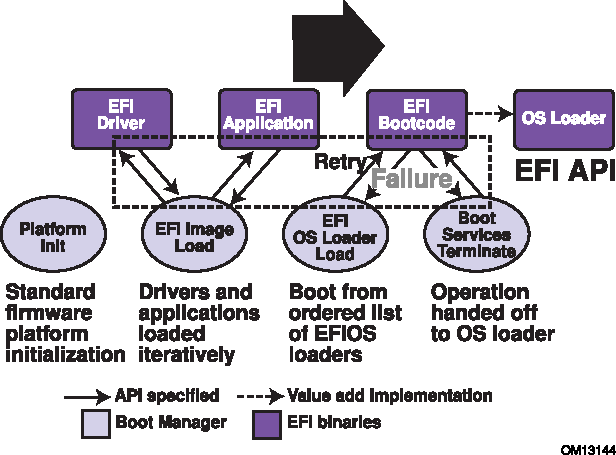
\includegraphics[width=\textwidth]{uefi_boot_sequence}%
    \caption{Booting Sequence\cite[Figure 2-1]{uefi-spec}}%
    \label{fig:uefi-boot-sequence}%
\end{figure}

\subsection{\ac{CSM}}


% !TeX root = ../../thesis.tex

\subsection{Secure Boot}

Secure Boot provides a secure hand-off from the firmware to 3rd party applications used for during the boot process, located on unsecure media \cite{tianocore-understanding-uefi-secure-boot-chain} \cite[Sections 32.2 and 32.5.1]{uefi-spec}.
It assumes the firmware to be a trusted entity and all 3rd party software to be untrusted, this includes images from hardware vendors in \ac{PCI} option \acp{ROM}, bootloader from \ac{OS} vendors and tools such as the \ac{UEFI} shell \cite{tianocore-understanding-uefi-secure-boot-chain}.
Digital signatures, embedded within the \ac{UEFI} images, can be used to authenticate origin and/or integrity \cite[Section 32.2]{uefi-spec}.
This is done through asymmetric signing, component provider must sign their executables with their private key and publish the public key.
The public keys are stored in a signature \ac{DB} and before execution the signed executable can be verified against the database.
Multiple signatures can be embedded within the same image \cite[Section 32.2.2]{uefi-spec}.
The signatures are created by first calculating a hash over select parts of the executable, leaving, for example, the signatures out of the hashed data and then signing it with a private key.
The output of this hashing is called a digest and the algorithm for obtaining the digest is defined in \cite{microsoft-pe-signature-format}.
Secure Boot also disallows legacy booting through the \ac{CSM}.

Secure Boot is managed through three components, a \ac{PK}, one or more \ac{KEK} and the signature \acp{DB}.

\begin{description}
    \item[\ac{PK}]
        The \ac{PK} establishes a trust relationship between platform owner and firmware, the public half is enrolled into the firmware.
        The private half represents platform ownership, as it can be used to change or delete the \ac{PK} as well as enroll or modify \acp{KEK}.
    \item[\ac{KEK}]
        The \ac{KEK} establishes a trust relationship between \ac{OS} and firmware, as its private half is used to modify the signature \acp{DB}.
    \item[Signature \acfp{DB}]
        Signature \acp{DB} contain image hashes and certificates, to either allow or deny execution of associated images.
\end{description}

Internally these are all implemented by authenticated variables, residing in tamper resistant non-volatile storage \cite[Section 32.3]{uefi-spec}.
The \ac{PK} is a simple variable where the \ac{KEK} and \ac{DB} are implemented through signature list data structures \cite[Section 32.4.1]{uefi-spec}, the variable services can be used to append entries or to read and write the list as a whole \cite[Sections 32.3.5 and 32.5.3]{uefi-spec}.
The variables are part of the \hyperref[sec:uefi-pi:uefi:variables]{Globally Defined Variables}, for each variavble also exist a variant reserved for default entries. These can be used by an \ac{OEM} to supply platform\-/defined values, used during Secure Boot initialization.
Their contents can be copied to their live versions, used during Secure Boot operation.
The current state of Secure Boot is also reflected within a secure variable \cite[Section 3.3]{uefi-spec}.

% https://papers.vx-underground.org/papers/Other/Advanced%20Malware/UEFI%20Secure%20Boot%20in%20Modern%20Computer%20Security%20Solutions.pdf
Users, who are physically present, may disable Secure Boot, enroll default or custom keys via an interactive menu. \TODO{find a good cite}

\TODO{maybe secure boot authorization process}

\subsection{Firmware Management}

\TODO{me}

% https://microsoft.github.io/mu/dyn/mu_tiano_plus/FmpDevicePkg/Docs/FmpDevicePkg_ReadMe/

provides
CapsuleUpdate()
QueryCapsuleCapabilities()
of the runtime services table